\documentclass[
    18pt,
    a0paper,
    landscape,
    margin=0mm,
    innermargin=18mm,
    blockverticalspace=8mm,
    colspace=12mm
]{tikzposter}

% =========================================================

\usepackage[T1]{fontenc}
\usepackage{amsmath}
\usepackage{amssymb}
\usepackage{booktabs}
\usepackage{array}
\usepackage{graphicx}
\usepackage{xcolor}
\usepackage{ragged2e}
\usepackage{hyperref}
\usepackage{url}
\usepackage{enumitem}

\setlength{\parindent}{0pt}
\setlist[itemize]{
    leftmargin=1.4em,
    itemsep=0.15em,
    topsep=0.2em,
    parsep=0pt
}

% ---------- Colour palette ----------
\definecolor{PosterGreen}{RGB}{45,105,55}
\definecolor{PosterText}{RGB}{35,35,35}
\definecolor{PosterGray}{RGB}{100,100,100}

\usetheme{Simple}
\titlegraphic{}
\useblockstyle{Minimal}

\colorlet{backgroundcolor}{white}
\colorlet{titlebgcolor}{white}
\colorlet{titlefgcolor}{PosterText}
\colorlet{blocktitlebgcolor}{white}
\colorlet{blocktitlefgcolor}{PosterGreen}
\colorlet{blockbodybgcolor}{white}
\colorlet{blockbodyfgcolor}{PosterText}
\colorlet{framecolor}{white}

% ---------- Title and block styling ----------
\definetitlestyle{GreenRule}{
    width=\paperwidth,
    roundedcorners=0,
    linewidth=0pt,
    innersep=12mm,
    titletotopverticalspace=9mm,
    titletoblockverticalspace=12mm
}{
    \draw[color=PosterGreen, line width=2.5pt]
        (\titleposleft, \titleposbottom-0.35cm)
        -- (\titleposright, \titleposbottom-0.35cm);
}
\usetitlestyle{GreenRule}

\renewcommand{\blocktitlefont}{\color{PosterGreen}\bfseries\Large}
\renewcommand{\arraystretch}{1.12}
\hypersetup{colorlinks=true, urlcolor=PosterGreen}

\newcommand{\headrule}{%
    \par\vspace{0.03cm}%
    {\color{PosterGreen}\rule{0.56\linewidth}{1pt}}%
    \par\vspace{0.14cm}%
}

\newcommand{\captiontext}[1]{%
    \par\vspace{0.05cm}\centering\scriptsize\color{PosterGray}#1\par
}

% ---------- Title ----------
\title{From-Scratch $\arccos(x)$ Calculator: Taylor Series, Newton's Method, and Software Quality Assurance}
\author{Mohammad Aliyawar Khan}
\institute{Department of Computer Science and Software Engineering, Concordia University \quad|\quad SOEN 6011 -- Deliverable 3 \quad|\quad Summer 2026}

\begin{document}
\maketitle

\begin{columns}

% =========================================================
% COLUMN 1 -- BACKGROUND AND NUMERICAL METHOD
% =========================================================
\column{0.25}

\block{Background}{
\headrule
\justifying
This project implements the principal real value of $\arccos(x)$ from
scratch in Python. The production calculation does not use library
inverse-trigonometric or square-root functions.

\textbf{Requirements}
\begin{itemize}
    \item Domain: $-1 \leq x \leq 1$
    \item Principal range: $[0,\pi]$ radians
    \item Tested absolute error: $\leq10^{-6}$ radians
    \item Tkinter GUI, helpful errors, and recovery
\end{itemize}

\textbf{D3 additions:} PEP~8, Flake8, Pylint, \texttt{pdb}, Semantic
Versioning, UIDP, accessibility, and PyUnit tests.
}

\block{Range Reduction and Taylor Series}{
\headrule
\justifying
Direct Taylor-series evaluation is slow near $\pm1$. For non-negative
input, the program uses
\[
\arccos(x)=2\arcsin\left(\sqrt{\frac{1-x}{2}}\right), \qquad x\geq0.
\]
For negative input,
\[
\arccos(x)=\pi-\arccos(-x), \qquad x<0.
\]
The reduced arcsine argument is near $0$ when $x$ is near $1$.
Endpoints return exact values: $\arccos(1)=0$ and $\arccos(-1)=\pi$.

\textbf{Taylor series}
\[
\arcsin(x)=\sum_{n=0}^{\infty}
\frac{(2n)!}{4^n(n!)^2(2n+1)}x^{2n+1}.
\]
A recurrence generates terms without repeatedly computing factorials.
The Taylor calculation stops when $|\mathrm{term}|\leq10^{-10}$ or
raises \texttt{ConvergenceError} after 1000 iterations.
}

\block{Newton Square-Root Method}{
\headrule
\justifying
The range-reduction square root is calculated from scratch using
Newton's method:
\[
g_{n+1}=\frac12\left(g_n+\frac{S}{g_n}\right).
\]
Tolerance: $10^{-14}$; maximum iterations: 100; initial guess: $1.0$.
}

\block{Final Tkinter GUI}{
\headrule
\justifying
The accessible Tkinter interface provides a labelled input field,
Calculate, Clear, and Exit controls, a result area, and a text-based
status message.

\begin{center}
\screenshot{gui-success.png}{3.5cm}
\captiontext{Exact endpoint calculation:
$\arccos(-1)=3.1415926536$ radians.}

\vspace{0.15cm}

\screenshot{gui-error.png}{3.5cm}
\captiontext{Helpful textual validation feedback; users can correct
input and calculate again without restarting.}
\end{center}
}
% =========================================================
% COLUMN 2 -- SOFTWARE QUALITY TOOLS
% =========================================================
\column{0.25}

\block{Implementation and Versioning}{
\headrule
\justifying
\textbf{From-scratch implementation.} The application manually
implements absolute value, square root, arcsine, and arccosine.
Tkinter is used only for the interface; \texttt{math} is not imported
by \texttt{problem7.py}.

\textbf{Validation and exceptions}
\begin{itemize}
    \item \texttt{InputValidationError}: NaN, infinity, or invalid domain
    \item \texttt{ConvergenceError}: configured iteration limit reached
    \item NaN is detected by $x\neq x$; infinity is rejected using a magnitude bound
\end{itemize}

\textbf{Semantic Versioning}
\[
\boxed{\texttt{\_\_version\_\_ = "1.0.0"} \Rightarrow \textbf{v1.0.0}}
\]
Version v1.0.0 is the first stable release; the same identifier is used
in the GUI title, README, and Git tag.
}

\block{PEP 8 and Flake8}{
\headrule
\justifying
Applied practices include four-space indentation, descriptive names,
docstrings, grouped constants, wrapped expressions, and separated
numerical and GUI responsibilities.

\begin{center}\ttfamily\small
python -m flake8 problem7.py test\_problem7.py
\end{center}

\begin{center}
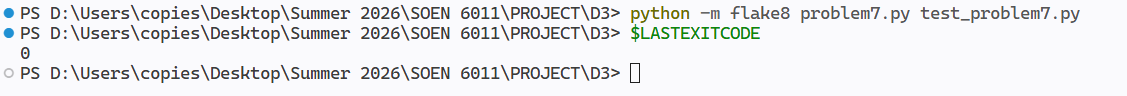
\includegraphics[width=0.94\linewidth,height=5.2cm,keepaspectratio]{flake8-result.png}
\captiontext{Flake8 execution on the final source and test files.}
\end{center}
}

\block{Static Analysis with Pylint}{
\headrule
\justifying
Pylint inspected the final code for errors, naming, documentation,
unused code, exception handling, and maintainability.

\begin{center}\ttfamily\small
python -m pylint problem7.py test\_problem7.py
\end{center}

\begin{center}
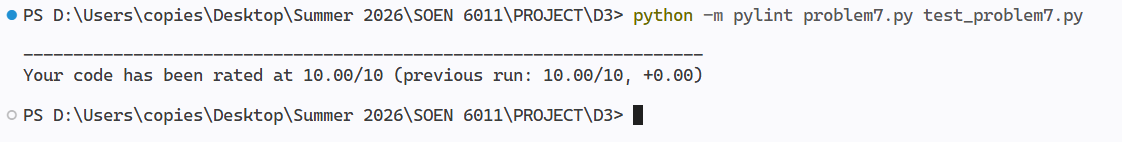
\includegraphics[width=0.94\linewidth,height=5.5cm,keepaspectratio]{pylint-result.png}
\captiontext{Pylint analysis report for the final files.}
\end{center}
}

% =========================================================
% COLUMN 3 -- DEBUGGING AND TESTING
% =========================================================
\column{0.20}

\block{Debugging with \texttt{pdb}}{
\headrule
\justifying
A near-endpoint calculation, $x=0.9999$, was stepped through to verify
range reduction and the Taylor recurrence. The session inspected
\texttt{x}, \texttt{reduced\_input}, \texttt{term}, \texttt{coefficient},
and \texttt{result}.

\begin{center}
\begin{tabular}{ll}
\toprule
\textbf{Command} & \textbf{Purpose}\\
\midrule
\texttt{n} & Execute next line\\
\texttt{s} & Step into function\\
\texttt{p variable} & Inspect variable\\
\texttt{c} & Continue execution\\
\bottomrule
\end{tabular}
\end{center}

\begin{center}
\includegraphics[width=0.94\linewidth,height=4.3cm,keepaspectratio]{pdb-session-a.png}
\captiontext{Debugger steps through validation and range reduction.}
\vspace{0.12cm}
\includegraphics[width=0.94\linewidth,height=4.3cm,keepaspectratio]{pdb-session-b.png}
\captiontext{Debugger inspects Taylor-series variables and final result.}
\end{center}
}

\block{Unit Testing -- Problem 8}{
\headrule
\justifying
The automated test suite uses Python's built-in \texttt{unittest}
framework (PyUnit) and imports the D3 module \texttt{problem7.py}.

\textbf{Coverage:} helper functions, Newton square root, Taylor
arcsine, exact endpoints, normal inputs, near-endpoint inputs, domain
violations, NaN, infinity, principal range, and numerical accuracy.

\begin{center}\ttfamily\small
python -m unittest -v test\_problem7.py
\end{center}

\begin{center}
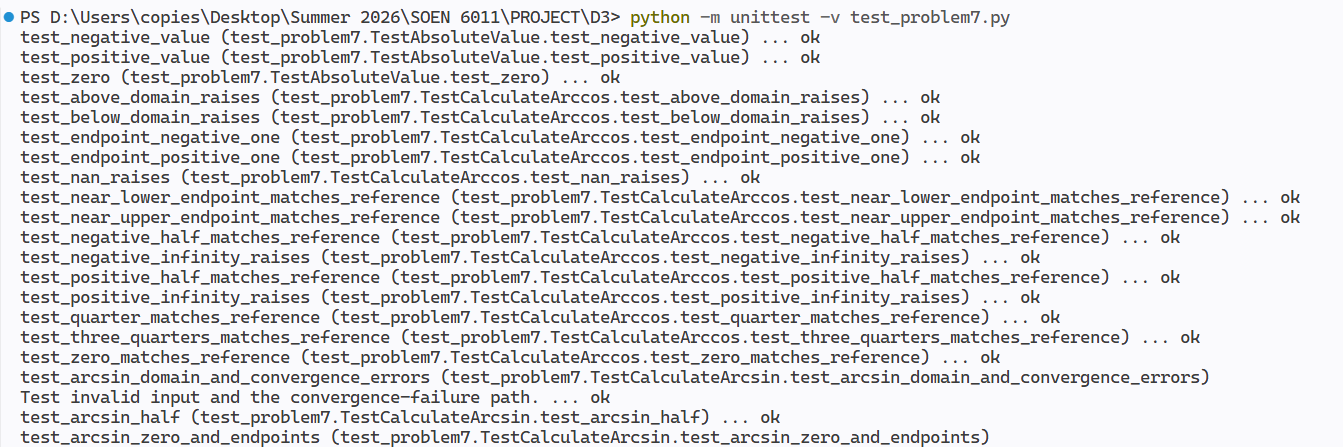
\includegraphics[width=0.94\linewidth,height=4.0cm,keepaspectratio]{testcase1.png}
\captiontext{PyUnit execution evidence: first group of test cases.}
\vspace{0.12cm}
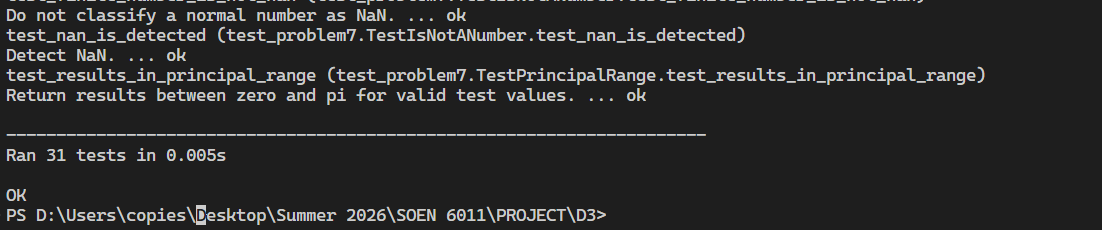
\includegraphics[width=0.94\linewidth,height=4.0cm,keepaspectratio]{testcase2.png}
\captiontext{PyUnit execution evidence: final tests and \texttt{OK} result.}
\end{center}
}

\block{Selected Test Cases}{
\headrule
\small
\begin{center}
\begin{tabular}{p{0.12\linewidth}p{0.25\linewidth}p{0.50\linewidth}}
\toprule
\textbf{ID} & \textbf{Input} & \textbf{Expected outcome}\\
\midrule
TC01 & $1.0$ & Exact result $0.0$\\
TC02 & $-1.0$ & Exact result $\pi$\\
TC03 & $0.0$ & Approximately $\pi/2$\\
TC04 & $0.5$ and $-0.5$ & Approximately $\pi/3$ and $2\pi/3$\\
TC05 & $\pm0.9999$ & Accurate near-endpoint result\\
TC06 & $1.1$, $-1.1$ & \texttt{InputValidationError}\\
TC07 & NaN, $\pm\infty$ & \texttt{InputValidationError}\\
TC08 & Valid test set & Error $\leq10^{-6}$ radians\\
\bottomrule
\end{tabular}
\end{center}
}

% =========================================================
% COLUMN 4 -- UIDP, GAI, CONCLUSION, REFERENCES
% =========================================================
\column{0.25}

\block{UIDP and Accessibility}{
\headrule
\justifying
The UIDP mind map selected principles appropriate for a single-purpose
scientific calculator.

\textbf{Applied}
\begin{itemize}
    \item Visible input, result, and textual status feedback
    \item Match with user language: $x$, radians, and $[-1,1]$
    \item Consistency, error prevention, and error recovery
    \item User control: Calculate, Clear, and Exit
    \item Keyboard access: Tab, Enter, Ctrl+L, and Ctrl+Q
    \item Readable fonts, high contrast, and resizable window
\end{itemize}

\textbf{Not applicable:} complex navigation, multi-window workflows,
drag-and-drop, user accounts, and undo/redo for persistent data.

\begin{center}
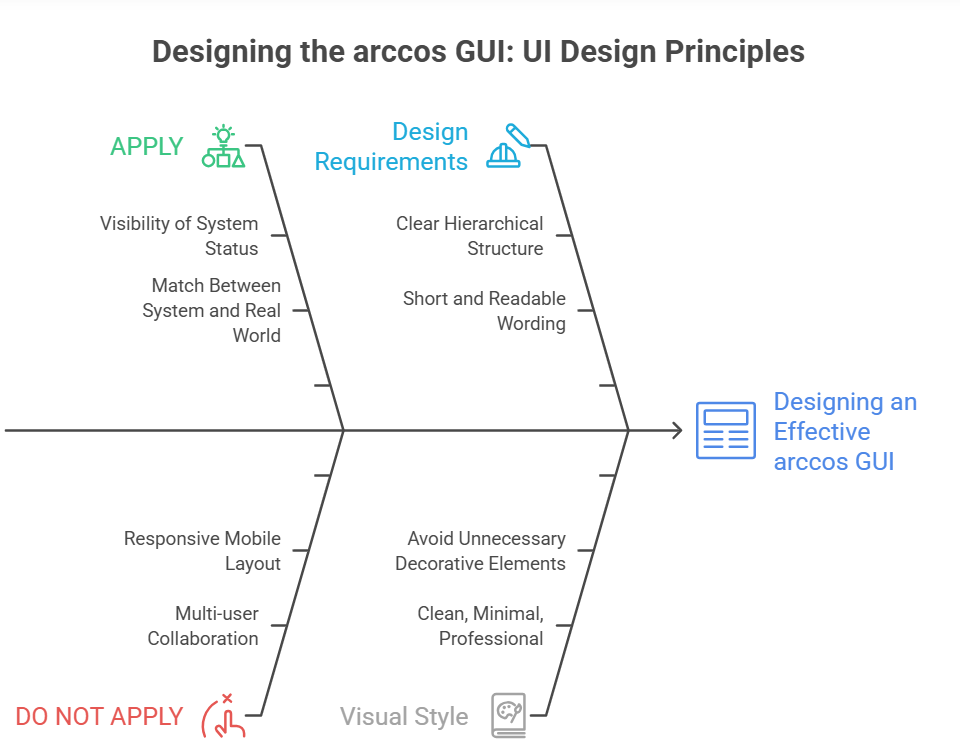
\includegraphics[width=0.94\linewidth,height=5.0cm,keepaspectratio]{uidp-mind-map.png}
\captiontext{UIDP applicability decision mind map.}
\end{center}
}

\block{GAI and CASTROFF Evidence}{
\headrule
\small\justifying
\textbf{Problem 7 prompt type:} code-quality and accessibility review.
The prompt supplied the from-scratch Tkinter context, requested PEP~8,
maintainability, UIDP, and accessibility improvements, prohibited
math-library functions, and required prioritized recommendations.

\textbf{Decision:} accepted clearer feedback, visible focus, keyboard
support, and documentation suggestions; rejected suggestions that would
violate the from-scratch constraint.

\textbf{Problem 8 prompt type:} boundary and exception-test review.
Suggested tests were validated against the final implementation and
executed locally.
}

\block{Conclusion}{
\headrule
\justifying
The D3 release combines a range-reduced Taylor series and Newton square
root with validation, exception recovery, and a Tkinter GUI. Flake8,
Pylint, \texttt{pdb}, Semantic Versioning, UIDP-based accessibility,
and automated PyUnit tests provide verifiable quality evidence.

\textbf{Result:} a numerically reliable, maintainable, testable, and
accessible $\arccos(x)$ calculator.
}

\block{References and Repository}{
\headrule
\scriptsize
[1] Concordia University, \emph{SOEN 6011 Project Description}, Summer 2026.\\
[2] Python Software Foundation, \emph{PEP 8}, \url{https://peps.python.org/pep-0008/}.\\
[3] PyCQA, \emph{Flake8}, \url{https://flake8.pycqa.org/}.\\
[4] Pylint Contributors, \emph{Pylint}, \url{https://pylint.readthedocs.io/}.\\
[5] Python Software Foundation, \emph{pdb}, \url{https://docs.python.org/3/library/pdb.html}.\\
[6] Python Software Foundation, \emph{unittest}, \url{https://docs.python.org/3/library/unittest.html}.\\
[7] Semantic Versioning, \url{https://semver.org/}.\\
[8] W3C, \emph{WCAG 2.2}, \url{https://www.w3.org/TR/WCAG22/}.

\vspace{0.18cm}
\normalsize\textbf{Repository:}\\
\ttfamily\small github.com/md-aliyawar-khan/\\
SOEN-6011-D3-arccos-calculator
}

\end{columns}
\end{document}